% Mini-project proposal
% Compile with XeLaTeX (needed for Devanagari):  xelatex proposal.tex  (run twice)
\documentclass[11pt,a4paper]{article}

\usepackage[margin=2.3cm]{geometry}
\usepackage{fontspec}
\usepackage{amsmath}
\usepackage{microtype}
\usepackage{booktabs,tabularx,array}
\usepackage[table]{xcolor}
\usepackage{enumitem}
\usepackage{caption}
\usepackage{float}
\usepackage{titlesec}
\usepackage{tikz}
\usetikzlibrary{positioning,arrows.meta}
\usepackage[colorlinks=true,linkcolor=accent,citecolor=accent,urlcolor=accent]{hyperref}

% ---------- Fonts ----------
\IfFontExistsTF{Noto Serif Devanagari}
  {\newfontfamily\devfont[Script=Devanagari,Scale=0.95]{Noto Serif Devanagari}}
  {\IfFontExistsTF{Devanagari MT}
    {\newfontfamily\devfont[Script=Devanagari]{Devanagari MT}}
    {\newfontfamily\devfont[Script=Devanagari]{Kohinoor Devanagari}}}
\newcommand{\hi}[1]{{\devfont #1}}

% ---------- Style ----------
\definecolor{accent}{HTML}{1F5F7A}
\definecolor{muted}{HTML}{5F6368}
\newcolumntype{Y}{>{\raggedright\arraybackslash}X}
\titleformat{\section}{\large\bfseries\color{accent}}{\thesection}{0.6em}{}
\titleformat{\subsection}{\normalsize\bfseries}{\thesubsection}{0.6em}{}
\titlespacing*{\section}{0pt}{1.2em}{0.5em}
\titlespacing*{\subsection}{0pt}{0.9em}{0.35em}
\setlist{itemsep=0.15em,topsep=0.3em}
\captionsetup{font=small,labelfont=bf}
\setlength{\parskip}{0.35em}
\setlength{\parindent}{0pt}
\renewcommand{\arraystretch}{1.15}
\tikzset{
  pstep/.style={draw=accent,rounded corners=3pt,fill=accent!6,
    minimum width=3.45cm,minimum height=1.15cm,align=center,font=\footnotesize},
  arr/.style={-{Stealth[length=2mm]},draw=accent,thick}
}
\newcommand{\refuted}[1]{\\{\small\textcolor{muted}{\emph{Refuted if} #1}}}

\begin{document}

% ======================================================= Title
\begin{center}
{\LARGE\bfseries Where Does the Model Look?}\\[0.4em]
{\large Localising Context-Driven Hindi Distinctions in Small Language Models}\\[1em]
{\normalsize Aaditya Bhatia \qquad Aryan Chaudhary}\\[0.2em]
{\small IIIT Hyderabad}\\[0.2em]
{\small Mechanistic Interpretability --- Mini-Project Proposal \quad$\cdot$\quad October 2026}
\end{center}

\vspace{0.4em}
\begin{abstract}
\noindent Hindi makes a model choose between forms that English collapses into one word: the speaker's gender in first-person verbs (\hi{गया}/\hi{गई}), the formality of ``you'' (\hi{आप}/\hi{तुम}/\hi{तू}), and the side of the family in kinship terms (\hi{मामा}/\hi{चाचा}). The information for each choice is not in the word itself; it has to come from the context. Benchmarks show that LLMs often get these choices wrong, but none explains why. We propose to find, in Gemma-3-4B, whether correct outputs are caused by the context cue or by a default prior, which positions, layers, heads and MLPs carry the cue to the answer, and whether failures happen because the cue is never encoded or because it is encoded but not used. We use causal methods only to support claims: activation patching, linear probes with control tasks, the logit lens with direct logit attribution, pre-trained sparse autoencoders, and steering. Sarvam-1, a 2B model built for Indian languages, is the fallback for any task Gemma-3-4B cannot do. No model training is needed beyond linear probes.
\end{abstract}

% ======================================================= 1
\section{Motivation}

Table~\ref{tab:english} shows three choices that Hindi forces and English does not. A model translating from English or writing Hindi has to recover each of them from the context: the speaker's name, the person being addressed, or the relative mentioned earlier.

\begin{table}[H]
\centering
\small
\begin{tabular}{@{}l l l l@{}}
\toprule
\textbf{English} & \textbf{Hindi must choose} & \textbf{Decided by} & \textbf{Cost of an error} \\
\midrule
I went & \hi{मैं गया} / \hi{मैं गई} & speaker's gender & misgenders the speaker \\
you & \hi{आप} / \hi{तुम} / \hi{तू} & addressee's status & rude to a teacher or an elder \\
uncle & \hi{चाचा} / \hi{मामा} / \hi{ताऊ} / \hi{फूफा} & side of family, generation & names the wrong relative \\
\bottomrule
\end{tabular}
\caption{Distinctions Hindi makes that English does not.}
\label{tab:english}
\end{table}

These errors have a social cost and appear both in translation from English and in Hindi generation. When a model gets one wrong, there are three possible causes, and each needs a different fix:
\begin{enumerate}[label=(\alph*)]
  \item the cue was \textbf{never encoded} in the model's activations, which needs more or better data;
  \item the cue was encoded but \textbf{not used} at the answer position (a \emph{readout failure}), which may be repairable at inference time;
  \item the cue was used but \textbf{overridden by a default}, such as a masculine or paternal form.
\end{enumerate}
Behavioural evaluation cannot tell these apart. Causal interpretability can.

% ======================================================= 2
\section{Related work and gap}

\paragraph{The failures are documented.}
Pardasani and Singh~\cite{pardasani2026} study kinship terms in Hindi, Tamil and Korean: GPT-OSS-120B \emph{picks} the right term 90.67\% of the time but \emph{produces} it only 36.00\% of the time, with a large paternal-side advantage in Hindi. MORPHOGEN~\cite{morphogen2026} finds clear gaps in first-person gender agreement in French, Arabic and Hindi across 15 LLMs from 2B to 70B parameters. A study of Hindi and Bengali honorifics~\cite{honorific2025} finds that LLMs use honorifics more often for men than for women. All three measure behaviour only; none asks why the model fails or where the missing information goes.

\paragraph{Interpretability has not reached these phenomena.}
Agreement circuits have been mapped for person and number~\cite{ferrando2024,gidi2026}, including in Hindi, and Hindi--Urdu agreement has been modelled as a search process~\cite{zhou2024}, but no work covers gender, kinship or honorifics. Work on the ``latent language'' of multilingual models~\cite{wendler2024} reads intermediate layers through lenses, but different lenses systematically disagree about what those layers contain~\cite{bayazit2026}; Indic-TunedLens~\cite{panchal2026} trains lenses specifically for Indian languages. Lens readings therefore need causal confirmation. The IOI circuit~\cite{wang2022} gives a template for our speaker-gender task: name-mover heads that copy a name from the context to the answer position.

\paragraph{Gap.} As far as we found, no published work localises any of the three distinctions inside a model.

% ======================================================= 3
\section{Problem statement}

\begin{quote}
When a small LLM makes these Hindi choices correctly, \textbf{which context cue causes it}, \textbf{where in the network} is that cue carried, and \textbf{why does it fail} when it fails?
\end{quote}

We study three tasks (Table~\ref{tab:tasks}). Each is posed as next-token prediction: the model sees a Hindi prompt and must produce the form that the context requires. Each clean prompt has a corrupt twin that changes only the cue and keeps the same token count, so every difference in the model's behaviour can be traced to the cue.

\begin{table}[H]
\centering
\small
\begin{tabularx}{\textwidth}{@{}l Y l Y l@{}}
\toprule
\textbf{Task} & \textbf{Prompt (model predicts \_\_\_)} & \textbf{Correct} & \textbf{Cue the model must use} & \textbf{Minimal-pair edit} \\
\midrule
Kinship terms & \hi{मेरी माँ के भाई को मैं \_\_\_ कहता हूँ} & \hi{मामा} & \hi{माँ} (maternal side) + \hi{भाई} (male) & \hi{माँ}$\to$\hi{पिता} (\hi{मामा}$\to$\hi{चाचा}) \\[2pt]
Speaker gender & \hi{सीमा ने कहा, "मैं कल बाज़ार \_\_\_} & \hi{गई} & speaker's name (\hi{सीमा}, female) & \hi{सीमा}$\to$\hi{राहुल} (\hi{गई}$\to$\hi{गया}) \\[2pt]
Honorifics & \hi{छात्र ने शिक्षक से पूछा, "\_\_\_} & \hi{आप} & addressee's status (\hi{शिक्षक}, a teacher) & \hi{शिक्षक}$\to$\hi{बेटा} (\hi{आप}$\to$\hi{तुम}) \\
\bottomrule
\end{tabularx}
\caption{The three tasks, with one clean prompt and its minimal-pair edit each.}
\label{tab:tasks}
\end{table}

% ======================================================= 4
\section{Research questions and hypotheses}

\begin{description}[leftmargin=0pt,itemsep=0.25em]
  \item[RQ1 -- Behaviour.] How accurate is the model on each task, and what are its systematic errors and defaults when no cue is given?
  \item[RQ2 -- Context vs prior.] When the output is correct, is it caused by the cue? Does swapping only the cue flip the output as it should?
  \item[RQ3 -- Localisation.] Which token positions, layers, attention heads and MLPs carry the cue to the prediction?
  \item[RQ4 -- Failure diagnosis.] When the model is wrong, is the cue missing from the residual stream, or present but not used? Can a targeted intervention repair the output?
\end{description}

Each hypothesis is stated with the result that would refute it.

\begin{description}[leftmargin=0pt,itemsep=0.35em]
  \item[H1 (readout failures).] Most failures are readout failures: the cue can be read from the model's activations but is not used. Steering along the cue direction repairs part of them.
  \refuted{the cue cannot be read at the answer position on wrong items, or steering at natural strength repairs no more items than random directions.}
  \item[H2 (two-step kinship).] For two-step kinship terms (\hi{पिता की बहन के पति} $\to$ \hi{फूफा}), the intermediate relative (\hi{बुआ}) is computed in the middle layers and causally used.
  \refuted{\hi{बुआ} cannot be read in the middle layers, or swapping it for \hi{मौसी} does not change the answer from \hi{फूफा} to \hi{मौसा}.}
  \item[H3 (defaults).] With no cue, the model defaults to masculine verbs and paternal kinship terms, and late MLPs write this default.
  \refuted{neutral prompts show no preference, or patching the late MLPs leaves the default in place (for example, because it comes from the direct path from embedding to output).}
  \item[H4 (speaker heads).] Speaker gender is fetched by a few mid-layer attention heads that attend from the answer position to the speaker's name, similar to name-mover heads in the IOI circuit.
  \refuted{no small set of heads restores the answer when patched, or, with a distractor name present, those heads copy the nearest name instead of the speaker.}
\end{description}

% ======================================================= 5
\section{Models}

\begin{table}[H]
\centering
\small
\begin{tabularx}{\textwidth}{@{}l l l Y Y@{}}
\toprule
\textbf{Model} & \textbf{Role} & \textbf{Size} & \textbf{Why we use it} & \textbf{Interpretability tools} \\
\midrule
Gemma-3-4B (pretrained)~\cite{gemma3} & main & 4B, 34 layers & Multilingual (140+ languages, including Hindi); the best Hindi tokenizer we tested & TransformerLens; Gemma Scope 2 SAEs on every layer~\cite{gemmascope2} \\[2pt]
Sarvam-1~\cite{sarvam1} & fallback & 2B, 28 layers & Built for 10 Indian languages and English; used by Indic-TunedLens & NNsight (Llama-style architecture); no SAEs \\
\bottomrule
\end{tabularx}
\caption{Models.}
\label{tab:models}
\end{table}

We use the \textbf{pretrained} Gemma-3-4B, not the instruction-tuned one, so that instruction tuning does not confound the mechanism, and we load only its text model.

\paragraph{Tokenizer check.} We checked the tokenizers on our target words. In Gemma-3-4B every verb, pronoun, postposition and adjective we need is a single token (\hi{गया/गई}, \hi{था/थी}, \hi{आप/तुम/तू}, \hi{ने/को/का/की/के}), so the speaker-gender and honorific tasks have single-token answers. \hi{मामा}, \hi{चाचा}, \hi{नाना} and \hi{दादा} are also single tokens. Other kinship terms take two, and where a pair shares a stem the second token decides gender (\hi{मौसा} = \hi{मौ} + \hi{सा}, \hi{मौसी} = \hi{मौ} + \hi{सी}). Sarvam-1 takes one or two tokens per kinship term. We dropped Gemma-2-2B (two to four tokens per kinship term and weaker Hindi) and Qwen2.5 (four to six tokens per word).

\paragraph{Go/no-go after week 1, per task.} If Gemma-3-4B gets fewer than half of a task's items right, or its cue swaps rarely flip the output, that task moves to Sarvam-1. Otherwise Gemma-3-4B stays the model for that task.

\paragraph{Compute.} Gemma-3-4B runs in bf16 on an L4 (24\,GB); we use an A100 only for large batched patching runs. Sarvam-1 fits on a free T4 in fp16.

% ======================================================= 6
\section{Datasets}

All items are templated and checked by both authors, who are native Hindi speakers. For every clean prompt there is a corrupt prompt that changes only the cue and keeps the same token count.

\begin{table}[H]
\centering
\small
\begin{tabularx}{\textwidth}{@{}l Y c >{\raggedright\arraybackslash}p{2.7cm}@{}}
\toprule
\textbf{Task} & \textbf{What varies} & \textbf{Size} & \textbf{Clean $\leftrightarrow$ corrupt} \\
\midrule
Kinship terms & 14 one-step relations (\hi{मामा, चाचा, ताऊ, बुआ, फूफा, मौसी, मौसा}, \dots) and 6 two-step ones; definition, English-context and short-story prompts & $\sim$800 & \hi{माँ}$\leftrightarrow$\hi{पिता}, \hi{भाई}$\leftrightarrow$\hi{बहन}, \hi{बड़े}$\leftrightarrow$\hi{छोटे} \\[2pt]
Speaker gender & 40 length-matched names (20 female, 20 male); cue type: quoted speaker, self-introduction, English source sentence, no cue; with and without a distractor name & $\sim$1,000 & \hi{सीमा}$\leftrightarrow$\hi{राहुल} \\[2pt]
Honorifics & 10 higher-status addressees (\hi{शिक्षक, दादी, डॉक्टर}, \dots) vs.\ 10 close or younger ones (\hi{बेटा, दोस्त, छोटा भाई}, \dots); speaker varied & $\sim$500 & \hi{शिक्षक}$\leftrightarrow$\hi{बेटा} \\
\bottomrule
\end{tabularx}
\caption{Hindi minimal-pair datasets ($\sim$2,300 items in total).}
\label{tab:data}
\end{table}

\begin{itemize}
  \item \textbf{Agreement.} Honorific items are kept only when both authors label them the same.
  \item \textbf{Answer tokens.} Leading spaces change the token. Directly after a quote mark, \hi{आप} and \hi{तुम} are different tokens from the mid-sentence \texttt{\textvisiblespace}\hi{आप} and \texttt{\textvisiblespace}\hi{तुम}, so we score the exact variant each template produces. \hi{गई} and \hi{गया} split into two tokens directly after a quote mark, so every template puts a space before the verb.
  \item \textbf{Splits.} Training and test splits are made by \textbf{name and template}, so that no result depends on memorising a particular name. Causal analyses use only items the model answers correctly on the clean prompt.
  \item \textbf{Sanity check.} Before any analysis we confirm that the attention and MLP outputs we read add up to the residual stream, since Gemma-3 adds extra normalisation around both.
\end{itemize}

% ======================================================= 7
\section{Methodology}

We run one shared causal pipeline for every task (Figure~\ref{fig:pipeline}). Attribution methods (lenses, attention weights, direct logit attribution) are used only to suggest where to look; every claim is backed by an intervention.

\begin{figure}[H]
\centering
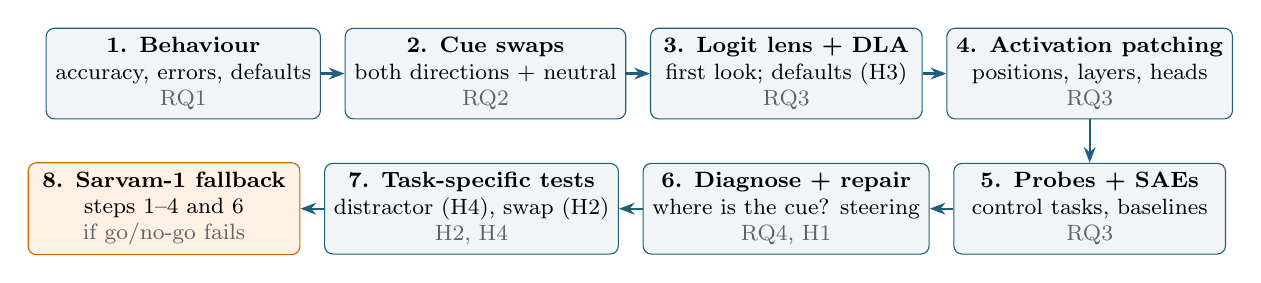
\begin{tikzpicture}[node distance=0.3cm]
  \node[pstep] (s1) {\textbf{1. Behaviour}\\accuracy, errors, defaults\\\textcolor{muted}{RQ1}};
  \node[pstep,right=of s1] (s2) {\textbf{2. Cue swaps}\\both directions + neutral\\\textcolor{muted}{RQ2}};
  \node[pstep,right=of s2] (s3) {\textbf{3. Logit lens + DLA}\\first look; defaults (H3)\\\textcolor{muted}{RQ3}};
  \node[pstep,right=of s3] (s4) {\textbf{4. Activation patching}\\positions, layers, heads\\\textcolor{muted}{RQ3}};
  \node[pstep,below=0.55cm of s4] (s5) {\textbf{5. Probes + SAEs}\\control tasks, baselines\\\textcolor{muted}{RQ3}};
  \node[pstep,left=of s5] (s6) {\textbf{6. Diagnose + repair}\\where is the cue? steering\\\textcolor{muted}{RQ4, H1}};
  \node[pstep,left=of s6] (s7) {\textbf{7. Task-specific tests}\\distractor (H4), swap (H2)\\\textcolor{muted}{H2, H4}};
  \node[pstep,left=of s7,fill=orange!10,draw=orange!80!black] (s8) {\textbf{8. Sarvam-1 fallback}\\steps 1--4 and 6\\\textcolor{muted}{if go/no-go fails}};
  \draw[arr] (s1) -- (s2); \draw[arr] (s2) -- (s3); \draw[arr] (s3) -- (s4);
  \draw[arr] (s4) -- (s5); \draw[arr] (s5) -- (s6); \draw[arr] (s6) -- (s7); \draw[arr] (s7) -- (s8);
\end{tikzpicture}
\caption{Experimental pipeline. The top row runs left to right, the bottom row right to left.}
\label{fig:pipeline}
\end{figure}

\subsection{Pipeline}

\begin{enumerate}[leftmargin=1.4em,itemsep=0.35em]
  \item \textbf{Behaviour (RQ1; both models).} Accuracy per task; an error matrix (wrong side of family, wrong gender, wrong generation); and the model's preferred output with the cue removed. We report forced-choice accuracy, top-1 and free generation, since picking the right form and producing it can differ. This step also decides, per task, whether Gemma-3-4B is good enough to analyse.
  \item \textbf{Context vs prior (RQ2).} Swap each cue word in both directions (female to male, and male to female) and replace it with a neutral cue. A swap that does not flip the answer means either that the prior dominates or that the new cue was not recognised. An asymmetry between the two directions is evidence for a default (H3).
  \item \textbf{Lenses and attribution (RQ3).} The logit lens for the correct vs.\ contrast token at every layer, used as a first look only: a weak early score can mean the information is absent or not yet aligned with the output space. Direct logit attribution identifies the heads and MLPs that push towards the default (H3); we check that the parts add up to the final score and confirm the result by patching.
  \item \textbf{Activation patching (RQ3).} Position $\times$ layer heatmaps on the residual stream, then attention vs.\ MLP outputs per layer, then individual heads. We patch in activations from the other run rather than zeroing them, and run both directions: restoring a component in the corrupt run (is it enough?) and replacing it in the clean run (is it needed?). The key result is the layer at which the effect moves from the cue position to the answer position.
  \item \textbf{Probes and SAE features (RQ3).} Linear probes for gender, side of family, relative age and addressee status at the answer position and every layer, with control tasks and baselines, trained and tested on different names and templates. The layer used later is chosen on a development split. Gemma Scope 2 features that fire on the cue or predict the output are ablated and steered, after checking that the SAEs reconstruct our prompts well.
  \item \textbf{Failure diagnosis and repair (RQ4; H1).} For wrong items, check where the cue can still be read: only at the cue position (it was never moved to the answer) or also at the answer position (moved but not used, or overridden by the default). Steer along both the probe direction and the difference-of-means direction at the localised layer, at a strength stated relative to the natural activation, and compare with random directions.
  \item \textbf{Task-specific tests.} \emph{Speaker gender:} a distractor name tests whether the model finds the speaker or just the nearest name; a candidate head must attend to the speaker's name, push directly towards the correct verb, and change the answer when patched (H4). \emph{Honorifics:} we check whether the verb that follows (\hi{हैं} vs.\ \hi{हो}) agrees with the pronoun the model chose. \emph{Kinship (stretch):} we read the intermediate term (\hi{बुआ}) in two-step prompts with the logit lens and Patchscopes~\cite{patchscopes2024}, then swap it for \hi{मौसी} and check that the answer changes from \hi{फूफा} to \hi{मौसा} (H2).
  \item \textbf{Sarvam-1 fallback.} A task that fails the week-1 go/no-go on Gemma-3-4B moves to Sarvam-1, where we run steps 1--4 and 6 in NNsight.
\end{enumerate}

\subsection{Metrics}

Causal metrics use only items the model answers correctly on the clean prompt. Every number is reported with a 95\% bootstrap interval that resamples whole templates, because items built from one template are not independent; comparisons on the same items use a paired interval on the difference.

\begin{description}[leftmargin=0pt,itemsep=0.4em]
  \item[Logit difference (LD).] How strongly the model prefers the correct form over its contrast at the answer position:
  \[ \mathrm{LD} = \mathrm{logit}(\text{correct}) - \mathrm{logit}(\text{contrast}), \quad\text{e.g. } \mathrm{logit}(\text{\hi{गई}}) - \mathrm{logit}(\text{\hi{गया}}). \]
  LD is the log of the probability ratio, so $\mathrm{LD}=2$ means \hi{गई} is about 7 times more likely than \hi{गया}. We use logits because each layer adds to them linearly, which lets the score be split across components. For two-token kinship terms we add the shared first token to the prompt and compare the second tokens (\hi{मौ} + \hi{सा} vs.\ \hi{मौ} + \hi{सी}), and also compare full-word log-probabilities.

  \item[Accuracy, top-1 and free generation.] Accuracy is the share of items with $\mathrm{LD}>0$. That does not mean the model would \emph{produce} the correct form, so we also report how often it is the top-1 prediction and how often it appears in free generation.

  \item[Flip rate.] Whether the answer comes from the cue. An item flips if $\mathrm{LD}_{\text{clean}}>0$ and $\mathrm{LD}_{\text{corrupt}}<0$, both measured in the same direction (e.g.\ \hi{गई} $-$ \hi{गया}):
  \[ \text{flip rate} = \frac{\#\,\text{flipped items}}{\#\,\text{items correct on clean}}, \]
  reported separately for each swap direction.

  \item[Patching effect.] How much one internal activation carries the cue. We rerun the corrupt prompt with one activation (a layer and position, a head, or an MLP) replaced by its value from the clean run:
  \[ \text{effect} = \frac{\mathrm{LD}_{\text{patched}} - \mathrm{LD}_{\text{corrupt}}}{\mathrm{LD}_{\text{clean}} - \mathrm{LD}_{\text{corrupt}}}. \]
  1 means that activation alone restores the clean behaviour; 0 means no effect. The reverse run (clean prompt, activation from the corrupt run) tests whether the activation is needed. LDs are averaged over items before dividing, and items where $\mathrm{LD}_{\text{clean}}-\mathrm{LD}_{\text{corrupt}}$ is near zero are dropped.

  \item[Probe accuracy and selectivity.] Whether a property (e.g.\ ``the speaker is female'') can be read linearly at a layer and position. A logistic-regression probe is trained on saved activations and scored on held-out names and templates. Following Hewitt and Liang~\cite{hewitt2019}, a control task gives each name a fixed random label, and
  \[ \text{selectivity} = \text{probe accuracy} - \text{control-task accuracy}. \]
  Majority-class, random-vector-per-word and layer-0 baselines are reported alongside. High accuracy with low selectivity means the probe is memorising words rather than reading the property.

  \item[Repair rate.] For wrong items, whether adding the cue direction fixes the output. We add $\alpha\,v$ to the residual stream at the localised layer, where $v$ is the unit-length probe or difference-of-means direction, and count items whose LD becomes positive:
  \[ \text{repair rate} = \frac{\#\,\text{repaired items}}{\#\,\text{wrong items}}. \]
  $\alpha$ is chosen on a development split and reported as a multiple of the natural activation along $v$. The baseline is the mean repair rate over 20 random directions of the same length, and items that were already right must stay right.

  \item[Logit lens and direct logit attribution (DLA).] The logit lens applies the final normalisation and unembedding to the residual stream at each layer and computes LD there, showing where the correct form starts to win. DLA projects each head's or MLP's output, scaled by the final normalisation, onto $W_U[\text{correct}] - W_U[\text{contrast}]$, giving its direct contribution to the final LD. The contributions must add up to the final LD before any part is interpreted. Gemma-3 applies no final logit soft-capping, so this decomposition is exact once the normalisation scale is fixed.
\end{description}

\subsection{What counts as evidence}

Table~\ref{tab:evidence} lists the claims the project could make and the evidence each one requires.

\begin{table}[H]
\centering
\small
\begin{tabularx}{\textwidth}{@{}>{\raggedright\arraybackslash}p{0.28\textwidth} Y@{}}
\toprule
\textbf{Claim} & \textbf{Required evidence} \\
\midrule
``The output comes from the context'' & The cue swap flips the output in both directions, and the patching effect moves from the cue position to the answer position across layers; this holds on held-out names and templates. \\[2pt]
``Component X carries the cue'' & Restoring X in the corrupt run brings back much of the LD, and replacing it in the clean run removes it, far more than for random components of the same size. A small effect from removal alone is inconclusive, since other components can compensate. \\[2pt]
``Head H fetches the speaker's gender'' & H attends to the speaker's name, pushes directly towards the correct verb, and changes the answer when patched, across many prompts and in the distractor test. \\[2pt]
``The distinction can be read at layer L'' & Probe selectivity above the control task and above the majority, random-vector and layer-0 baselines, on held-out names and templates, with L chosen on a development split. \\[2pt]
``The model uses that information'' & An intervention at L (removing or steering the direction) changes the output. \\[2pt]
``The failure is a readout failure'' & The cue can be read at the answer position on wrong items, and steering at natural strength repairs them clearly more often than random directions, without flipping items that were already right. \\
\bottomrule
\end{tabularx}
\caption{Claims and the evidence each one requires.}
\label{tab:evidence}
\end{table}

% ======================================================= 8
\section{Expected outcomes and impact}

\begin{itemize}
  \item \textbf{Fixable or not.} If a failure is a readout failure (the cue is present but unused), it can be repaired at inference time; if the cue is never encoded, it needs data. Our diagnosis separates the two.
  \item \textbf{Bias, located.} The masculine and paternal defaults (H3) let us trace where in the network a bias is written, not only that it exists.
  \item \textbf{First causal account} of kinship terms, speaker gender and honorifics in Hindi, and a test of whether IOI-style mechanisms appear outside English.
  \item \textbf{A per-task behavioural comparison} of Gemma-3-4B with Sarvam-1, a model built for Indian languages.
  \item \textbf{Released resources:} a verified Hindi minimal-pair dataset and reproducible notebooks.
\end{itemize}

% ======================================================= 9
\section{Timeline, priorities and risks}

The plan runs for four weeks, with a checkpoint at the end of each of the first three.

\begin{table}[H]
\centering
\small
\begin{tabularx}{\textwidth}{@{}l l Y Y@{}}
\toprule
\textbf{Week} & \textbf{Focus} & \textbf{Work} & \textbf{Checkpoint} \\
\midrule
1 & RQ1, RQ2 & Build and verify data; behaviour and cue swaps on Gemma-3-4B & Data ready; go/no-go per task \\
2 & RQ3 & Logit lens, DLA, activation patching (positions, layers, heads) & Localisation results \\
3 & RQ3 & Probes with control tasks; Gemma Scope 2 features & Probe and SAE results \\
4 & RQ4 & Failure diagnosis, steering and repair; task-specific tests; write-up & Final report and presentation \\
\bottomrule
\end{tabularx}
\caption{Four-week plan.}
\label{tab:timeline}
\end{table}

\textbf{Priority order.} \emph{Must:} speaker gender, steps 1--7 on Gemma-3-4B. \emph{Should:} honorifics; one-step kinship terms. \emph{Stretch:} two-step kinship terms (H2); a full Sarvam-1 comparison beyond the fallback.

\textbf{Progress so far.} The literature review is done and the three tasks are fixed. The tokenizers of Gemma-3-4B, Gemma-2-2B, Sarvam-1, Llama-3.2-1B, Qwen2.5-1.5B and BLOOM-1b1 have been checked on our target words, and tool support for Gemma-3-4B (TransformerLens, Gemma Scope 2) is confirmed. Prompt formats and clean/corrupt edits are drafted for all three tasks.

\begin{table}[H]
\centering
\small
\begin{tabularx}{\textwidth}{@{}>{\raggedright\arraybackslash}p{0.4\textwidth} Y@{}}
\toprule
\textbf{Risk} & \textbf{Mitigation} \\
\midrule
Gemma-3-4B is weak on a task (most likely kinship terms) & Analyse only correctly answered items; move that task to Sarvam-1 \\
Kinship terms span several tokens & LD at the first token where the two terms differ, plus full-word log-probability \\
Clean and corrupt prompts differ in length & Length-matched names and cue words; every pair checked with the tokenizer \\
Honorific choice is partly subjective & Clear status contrasts; keep only items both authors label the same \\
Gemma Scope 2 SAEs reconstruct Hindi poorly & Check reconstruction error on our prompts first; fall back to probe directions \\
High probe accuracy without a causal role & Control tasks for selectivity; every probe finding confirmed by patching or steering \\
The cue is spread over many components & Report patching maps honestly; a distributed mechanism is still a result \\
Sarvam-1 has no SAEs or TransformerLens support & NNsight for patching and steering; probe directions instead of SAE features \\
Steering strong enough to force any output & Strength as a multiple of the natural activation; random-direction baseline; correct items must stay correct \\
The answer token depends on spacing & Score the exact token each template produces; keep a space before the verb \\
Four weeks is tight & Priority order above; speaker gender finished end to end first \\
\bottomrule
\end{tabularx}
\caption{Risks and mitigations.}
\label{tab:risks}
\end{table}

% ======================================================= 10
\section{Deliverables}

\begin{itemize}
  \item A verified Hindi minimal-pair dataset for the three tasks ($\sim$2,300 items).
  \item Code notebooks (TransformerLens and NNsight) that reproduce every experiment.
  \item Results: patching heatmaps, layer-wise probe curves, SAE feature lists and repair rates.
  \item A final report and presentation.
\end{itemize}

% ======================================================= References
\begin{thebibliography}{99}
\small
\setlength{\itemsep}{0.15em}

\bibitem{pardasani2026} Pardasani and Singh. Recognized but Not Produced: A Generation Benchmark for Culturally Specific Kinship Terms. EMNLP 2026 ORACLE Workshop. \url{https://arxiv.org/abs/2609.26942}

\bibitem{morphogen2026} MORPHOGEN: A Multilingual Benchmark for Evaluating Gender-Aware Morphological Generation. ACL 2026. \url{https://preview.aclanthology.org/ingest-acl/2026.acl-long.105/}

\bibitem{honorific2025} Women, Infamous, and Exotic Beings: Honorific Usages in Wikipedia and LLMs for Bengali and Hindi. 2025. \url{https://arxiv.org/abs/2501.03479}

\bibitem{wang2022} Wang et al. Interpretability in the Wild: a Circuit for Indirect Object Identification in GPT-2 small. 2022. \url{https://arxiv.org/abs/2211.00593}

\bibitem{ferrando2024} Ferrando and Costa-juss\`a. On the Similarity of Circuits across Languages: Subject-Verb Agreement. EMNLP Findings 2024. \url{https://arxiv.org/abs/2410.06496}

\bibitem{gidi2026} Gidi et al. Shared Circuits for Shared Grammar: Tracing Subject-Verb Agreement Across Languages. COLM 2026. \url{https://arxiv.org/abs/2608.18545}

\bibitem{zhou2024} Zhou and Wilson. Modeling Morphosyntactic Agreement as Neural Search: Hindi-Urdu. SCiL 2024. \url{https://aclanthology.org/2024.scil-1.21.pdf}

\bibitem{patchscopes2024} Ghandeharioun et al. Patchscopes: A Unifying Framework for Inspecting Hidden Representations of Language Models. 2024. \url{https://arxiv.org/abs/2401.06102}

\bibitem{hewitt2019} Hewitt and Liang. Designing and Interpreting Probes with Control Tasks. EMNLP 2019. \url{https://arxiv.org/abs/1909.03368}

\bibitem{gemmascope2} Google DeepMind. Gemma Scope 2: SAEs for Gemma 3. 2025. \url{https://huggingface.co/google/gemma-scope-2-4b-pt}

\bibitem{wendler2024} Wendler et al. Do Llamas Work in English? On the Latent Language of Multilingual Transformers. ACL 2024. \url{https://arxiv.org/abs/2402.10588}

\bibitem{bayazit2026} Bayazit, AlKhamissi and Bosselut. Lingua Franca or Probing Artifact? Rethinking Latent Language in Multilingual LLMs. EMNLP Findings 2026. \url{https://arxiv.org/abs/2609.00155}

\bibitem{panchal2026} Panchal et al. Indic-TunedLens: Interpreting Multilingual Models in Indian Languages. VarDial @ EACL 2026. \url{https://arxiv.org/abs/2602.15038}

\bibitem{gemma3} Gemma Team. Gemma 3 Technical Report. 2025. \url{https://arxiv.org/abs/2503.19786}. Model: \url{https://huggingface.co/google/gemma-3-4b-pt}

\bibitem{sarvam1} Sarvam AI. Sarvam-1. 2024. \url{https://huggingface.co/sarvamai/sarvam-1}

\end{thebibliography}

\end{document}
